\subsection{Divergenca bivariatnih in multivariatnih porazdelitev}

Do sedaj smo obravnavali divergenco univariatnih porazdelitev, torej gostota verjetnosti je bila funkcija ene spremenljivke (npr. P porazdelitev, $p: \RR \rightarrow \RR$ njena gostota verjetnosti). Kaj pa če gledamo porazdelitve v več dimenzijah? Za začetek si poglejmo zgled.

\begin{zgled}
    Poglejmo si zgled bivariatne normalne porazdelitve. Kot primer v vsakdanjem življenju lahko vzamemo npr. populacijo ljudi in hkrati gledamo višino in težo.
    \begin{figure}[!ht]
        \centering
        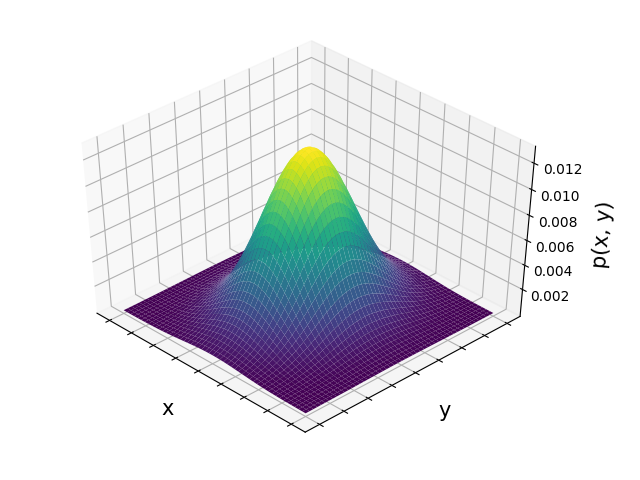
\includegraphics[width=\textwidth]{gauss-bivariate}
        \caption{Normalna porazdelitev v dveh dimenzijah.}
    \end{figure}
\end{zgled}

Izpustimo definicije in ostale primere porazdelitev, poglejmo raje, kako definiramo divergenco.
\pagebreak
Definicija divergence za bi- in multivariate porazdelitve sovpada z definicijo divergence za univariatne porazdelitve:
\begin{enumerate}
	\item $D(p \| q) \geq 0$ za vsaka $p, q \in S$, kjer je $S$ množica porazdelitev,
	\item $D(p \| q) = 0 \Leftrightarrow p = q$.
\end{enumerate}

Recimo, da gledamo porazdelitve v $n$ dimenzijah. Gostote verjetnosti teh porazdelitev bodo funkcije $p: \Omega \subseteq \RR^n \rightarrow \RR^+$. Divergence se torej na naraven način prevedejo za $n$-dimenzionalne porazdelitve. Poglejmo si to na primerih.

\begin{zgled}
    Naj bo $x=(x_1, x_2, \dots , x_n) \in \RR^n$. Naj bodo $p, q$ gostote verjetnosti z definicijskim območjem $\Omega \subseteq \RR^n$. Definicije divergenc razširimo na $n$ dimenzij:
	\begin{enumerate}
		\item \textbf{Kullback-Leiblerjeva divergenca}
		\begin{equation}
			D_{KL}(p \| q) = \idotsint\limits_\Omega p(x) \cdot \log\Big(\frac{p(x)}{q(x)}\Big) \  dx_1\dots dx_n.
		\end{equation}
		\item \textbf{f-divergenca}
		\begin{equation}
			D_f(p \| q) = \idotsint\limits_\Omega p(x) \cdot f\Big(\frac{p(x)}{q(x)}\Big) \  dx_1\dots dx_n.
		\end{equation}
		\item \textbf{Hellingerjeva distanca}
		\begin{equation}
			H^2(p, q) = 2 \cdot \idotsint\limits_\Omega \Big(\sqrt{p(x)} - \sqrt{q(x)}\Big)^2 \  dx_1\dots dx_n.
		\end{equation}
		\item \textbf{Renyi divergenca}
		\begin{equation}
			D_{\alpha}(p \| q)=\frac{1}{\alpha-1} \cdot \log \Bigg(\idotsint\limits_\Omega \Big(p(x)\Big)^{\alpha}\Big(q(x)\Big)^{1-\alpha}\  dx_1\dots dx_n\Bigg), \quad \quad \alpha \neq 1.
		\end{equation}
	\end{enumerate}
\end{zgled}